\documentclass{article}
%%Para esconder subsecciones en el índice:
%\setcounter{tocdepth}{1}


%Microtype
\usepackage[activate={true,nocompatibility},final,tracking=true,kerning=true,spacing=true,factor=1100,stretch=10,shrink=10]{microtype}
% activate={true,nocompatibility} - activate protrusion and expansion
% final - enable microtype; use "draft" to disable
% tracking=true, kerning=true, spacing=true - activate these techniques
% factor=1100 - add 10% to the protrusion amount (default is 1000)
% stretch=10, shrink=10 - reduce stretchability/shrinkability (default is 20/20)
\microtypecontext{spacing=nonfrench}
  \usepackage{pgfplots}
  \pgfplotsset{compat=newest}
  %% the following commands are needed for some matlab2tikz features
  \usetikzlibrary{plotmarks}
  \usetikzlibrary{arrows.meta}
  \usepgfplotslibrary{patchplots}
  \usepackage{grffile}
  %% Language and font encodings
\usepackage[english, spanish]{babel}
\usepackage[utf8]{inputenc}
\usepackage[T1]{fontenc}


% Sets page size and margins
\usepackage[a4paper,top=3cm,bottom=2cm,left=2.7cm,right=2.7cm,marginparwidth=2cm]{geometry}
%Para los gráficos
\definecolor{mycolor1}{rgb}{0.00000,0.44706,0.74118}%
\definecolor{mycolor2}{RGB}{255,165,0}%
\definecolor{rojo}{RGB}{255,0,0}%
\definecolor{verde}{RGB}{50,205,90}%
\definecolor{azulfrancia}{rgb}{0.00000,0.44706,0.74118}%
\definecolor{boston}{rgb}{0.8, 0.0, 0.0}
\usepackage{float}

%Tabla
\usepackage{booktabs}% http://ctan.org/pkg/booktabs
\usepackage{xcolor}
\usepackage{graphicx}
\usepackage{colortbl}
\usepackage{array}
\usepackage{pifont}
\usepackage{tabularx}

%% Useful packages
\usepackage{parskip}
\usepackage{pdflscape}
\usepackage{amsmath}
\usepackage{graphicx}
\usepackage[makeroom]{cancel}
\usepackage{tikz}
\usepackage{amssymb}
\usepackage[version=4]{mhchem}
\usepackage{textcomp}
\usepackage{gensymb}
\usepackage{circuitikz}
\usepackage{multicol}
\usepackage{caption}
\usepackage[colorinlistoftodos]{todonotes}
\usepackage[colorlinks=true, allcolors=black]{hyperref}
\usepackage[
backend=biber, style=ieee
]{biblatex}
\addbibresource{bibliografia.bib}

  %% you may also want the following commands
  %\pgfplotsset{plot coordinates/math parser=false}
  %\newlength\figureheight
  %\newlength\figurewidth
\usepackage{verbatim}
\usepackage[nodisplayskipstretch]{setspace}
\setstretch{1.2}
\usepackage{multicol}
\usepackage{caption}
\usepackage{subcaption}
\usepackage{chemfig}
\usepackage{geometry}
\usepackage{enumitem}
\usepackage{multirow}
\usepackage[ampersand]{easylist}
\title{Capitulo 2 - Circuitos Cerrados}
\author{Nicolás Goldman}
\date{March 2020}
\begin{document}

\maketitle

\section{Circuitos}
\subsection{DOLMEN}
\subsubsection*{Información general}
\textit{Nombre de la instalación: }DOLMEN (Double Latitude pour Maintenance En sodium)

\textit{Refrigerante: }Sodio

\textit{Ubicación: }CEA Cadarache

\textit{Inicio de operación: }1980, reformado en 2013/2014

\subsubsection*{Estado}
En operación

\subsubsection*{Campo de I\&D}
\begin{itemize}
\item[$\square$] Instalación de potencia cero para V \& V y propósitos de licencia
\item[$\square$] Design Basis Accidents (DBA) y Design Extended Conditions (DEC)
\item[$\square$] Termohidráulica
\item[$\square$] Química del refrigerante
\item[$\square$] Materiales
\item[$\boxtimes$] Sistemas y componentes
\item[$\boxtimes$] Instrumentación \& ISI\&R
\end{itemize}
\subsubsection*{Descripción técnica}
Esta instalación se utiliza para el ensayo de instrumentación, componentes pequeños y técnicas de reparación de sodio, telemetría de sodio, visualización de sodio. Además, se puede utilizar para preparar muestras para experimentos en otros equipos, por inmersión y mojado en sodio.

La instalación está compuesta por dos secciones de ensayo principales (T-1 de 1500L y T-2 de 600L), y puede alcanzar 600\celsius. El sodio utilizado tiene alta calidad química, obtenida mediante un sistema de purificación.
\subsubsection*{Esquema}
\begin{figure}[H]
\begin{center}
\frame{\includegraphics[width=0.8\paperwidth,keepaspectratio]{dolmen.pdf}}
\end{center}
\caption{Circuito DOLMEN}
\end{figure}
\subsubsection*{Foto}
\begin{figure}[H]
\begin{center}
\frame{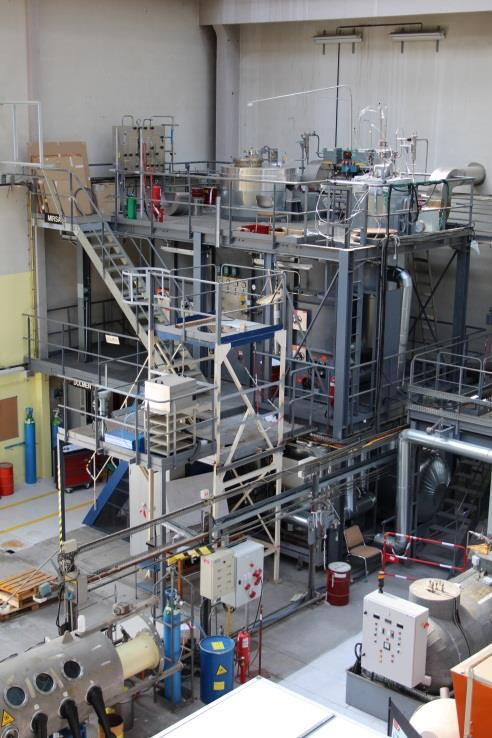
\includegraphics[width=0.45\paperwidth,keepaspectratio]{dolmen_foto.jpg}}
\end{center}
\caption{Foto de DOLMEN}
\end{figure}
\subsubsection*{Componentes}
\begin{table}[H]
\centering
\begin{tabular}{cp{3.5cm}}
\toprule
Código & Equipo \\
\midrule
B-01 & \multirow{2}{*}{Bomba} \\
B-02 & \\
\midrule
TK-01 & \multirow{2}{*}{Tanque de ensayos} \\
TK-02 & \\
\midrule
TK-03 & Tanque de \newline almacenamiento \\
\midrule
V-01 & \multirow{8}{*}{Válvula esclusa} \\
V-02 & \\
V-03 & \\
V-04 & \\
V-05 & \\
V-06 & \\
V-07 & \\
V-08 & \\
\midrule
VE-01 & \multirow{5}{*}{Venteo} \\
VE-02 & \\
VE-03 & \\
VE-04 & \\
VE-05 & \\
\midrule
& Presurizador \\
\midrule
& Sistema de purificación de sodio \\
\bottomrule
\end{tabular}
\end{table}
\subsubsection*{Variables de proceso}
\begin{table}[H]
\centering
\begin{tabular}{cp{3.5cm}}
\toprule
Presión & 0 $barg$ \\
Temperatura & $250\celsius\leqslant T \leqslant 600\celsius$ \\
Caudal & $1500$ $L/h$ (ambas \newline secciones) \\
Potencia & 70 $kW$ \\
\bottomrule
\end{tabular}
\end{table}
\subsubsection*{Campañas experimentales y resultados}
\begin{itemize}
    \item Técnicas de reparación de sodio
    \item Pruebas de proceso de carbonación
    \item Evaluación de desempeño de telemetría con técnicas de ultrasonido
    \item Evaluación de transductores de alta temperatura (hasta 600\celsius)
    \item Calibración de sondas de nivel inductivas
\end{itemize}
\subsubsection*{Experimentos planeados}
Establecer el desempeño de varios equipos de instrumentación de sodio: transductores nuevos de alta temperatura, transductores ultrasónicos de matriz en fases, transductores electromagnéticos, y también experimentos para demostrar la habilidad de hacer visualización de sodio.

A largo plazo, DOLMEN será usado para el ensayo de técnicas de reparación de sodio.
\subsubsection*{Actividades de entrenamiento}
No está planificado un programa específico
\newpage
\subsection{Circuito de bombas}
\subsubsection*{Información general}
\textit{Nombre de la instalación: }Circuito Cerrado Experimental de Bombas en Serie y Paralelo
\textit{Refrigerante: }Agua
\textit{Ubicación: }Ciudad Universitaria - Pabellón Industrias
\textit{Inicio de operación: }?
\subsubsection*{Estado}
En operación
\subsubsection*{Campo de I\&D}
No aplica
\begin{itemize}
\item[$\square$] Instalación de potencia cero para V \& V y propósitos de licencia
\item[$\square$] Design Basis Accidents (DBA) y Design Extended Conditions (DEC)
\item[$\square$] Termohidráulica
\item[$\square$] Química del refrigerante
\item[$\square$] Materiales
\item[$\boxtimes$] Sistemas y componentes
\item[$\square$] Instrumentación \& ISI\&R
\end{itemize}
\subsubsection*{Descripción técnica}
Este circuito se utiliza con fines didácticos; para obtener los parámetros de las curvas de altura de las bombas, y comparar la operación de las bombas individuales a distintas frecuencias, y en configuraciones serie y paralelo.
\subsubsection*{Esquema}
\begin{figure}[H]
\begin{center}
\frame{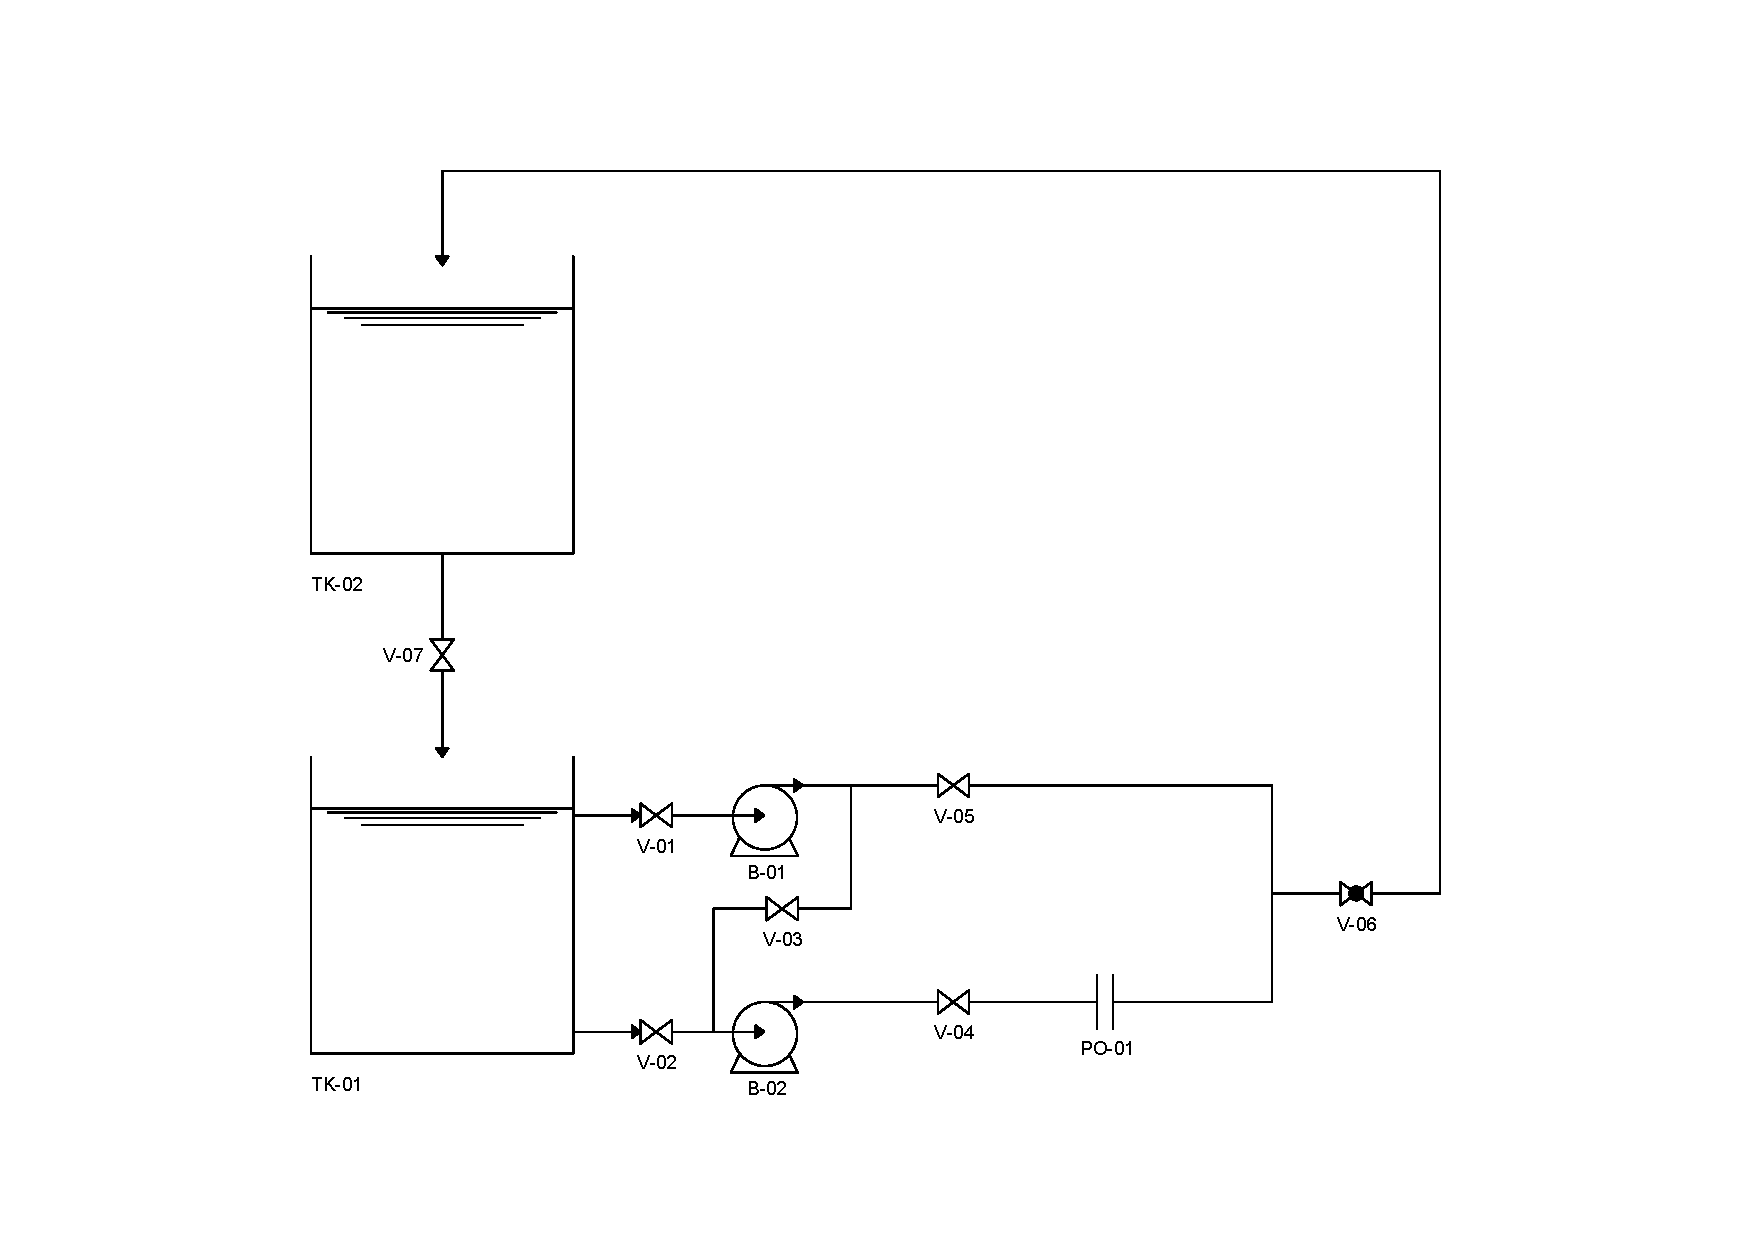
\includegraphics[width=0.8\paperwidth,keepaspectratio]{bombas.pdf}}
\end{center}
\caption{Circuito de bombas}
\end{figure}
\subsubsection*{Foto}
\begin{figure}[H]
\begin{center}
\frame{\includegraphics[width=0.8\paperwidth,keepaspectratio]{example-image.jpg}}
\end{center}
\caption{Foto del Circuito de bombas}
\end{figure}
\subsubsection*{Componentes}
\begin{table}[H]
\centering
\begin{tabular}{cp{3.5cm}}
\toprule
Código & Equipo \\
\midrule
B-01 & \multirow{2}{*}{Bomba} \\
B-02 & \\
\midrule
TK-01 & \multirow{2}{*}{Tanque} \\
TK-02 & \\
\midrule
V-01 & \multirow{6}{*}{Válvula esclusa} \\
V-02 & \\
V-03 & \\
V-04 & \\
V-05 & \\
V-07 & \\
\midrule
V-06 & Válvula globo \\
\midrule
PO-01 & Placa orificio \\
\bottomrule
\end{tabular}
\end{table}
\subsubsection*{Variables de proceso}
\begin{table}[H]
\centering
\begin{tabular}{cp{3.5cm}}
\toprule
Presión & $\leqslant 450$ $mbarg$ \\
Temperatura & 25\celsius \\
Caudal & $\leqslant 3.5$ $L/s$ \\
Potencia & No aplica \\
\bottomrule
\end{tabular}
\end{table}
\subsubsection*{Campañas experimentales y resultados}
\begin{itemize}
    \item Obtención de las curvas de operación de las bombas B-1 y B-2
    \item Obtención de las curvas de operación de las bombas en serie y en paralelo. El arreglo en serie permite lograr alturas mayores, y el arreglo en paralelo caudales mayores. Se encuentra un error alto en el arreglo en paralelo respecto de los valores teóricos, por la asimetría de las líneas
    \item Verificación de las leyes de afinidad para distintos diámetros y velocidades del rotor
\end{itemize}
%\subsubsection*{Experimentos planeados}
%Establecer el desempeño de varios equipos de instrumentación de sodio: transductores nuevos de alta temperatura, transductores ultrasónicos de matriz en fases, transductores electromagnéticos, y también experimentos para demostrar la habilidad de hacer visualización de sodio.

%A largo plazo, DOLMEN será usado para el ensayo de técnicas de reparación de sodio.
\subsubsection*{Actividades de entrenamiento}
No está planificado un programa específico
\newpage
\subsection{Circuito de pérdida de carga}
\subsubsection*{Información general}
\textit{Nombre de la instalación: }Circuito Cerrado Experimental de Pérdida de carga

\textit{Refrigerante: }Agua

\textit{Ubicación: }Ciudad Universitaria - Pabellón Industrias

\textit{Inicio de operación: }?

\subsubsection*{Estado}
En operación

\subsubsection*{Campo de I\&D}
\begin{itemize}
\item[$\square$] Instalación de potencia cero para V \& V y propósitos de licencia
\item[$\square$] Design Basis Accidents (DBA) y Design Extended Conditions (DEC)
\item[$\square$] Termohidráulica
\item[$\square$] Química del refrigerante
\item[$\square$] Materiales
\item[$\boxtimes$] Sistemas y componentes
\item[$\square$] Instrumentación \& ISI\&R
\end{itemize}
\subsubsection*{Descripción técnica}
Este circuito se utiliza con fines didácticos: con él se calibra el Venturi, y se comparan las pérdidas de carga de los equipos presentes.
\subsubsection*{Esquema}
\begin{figure}[H]
\begin{center}
\frame{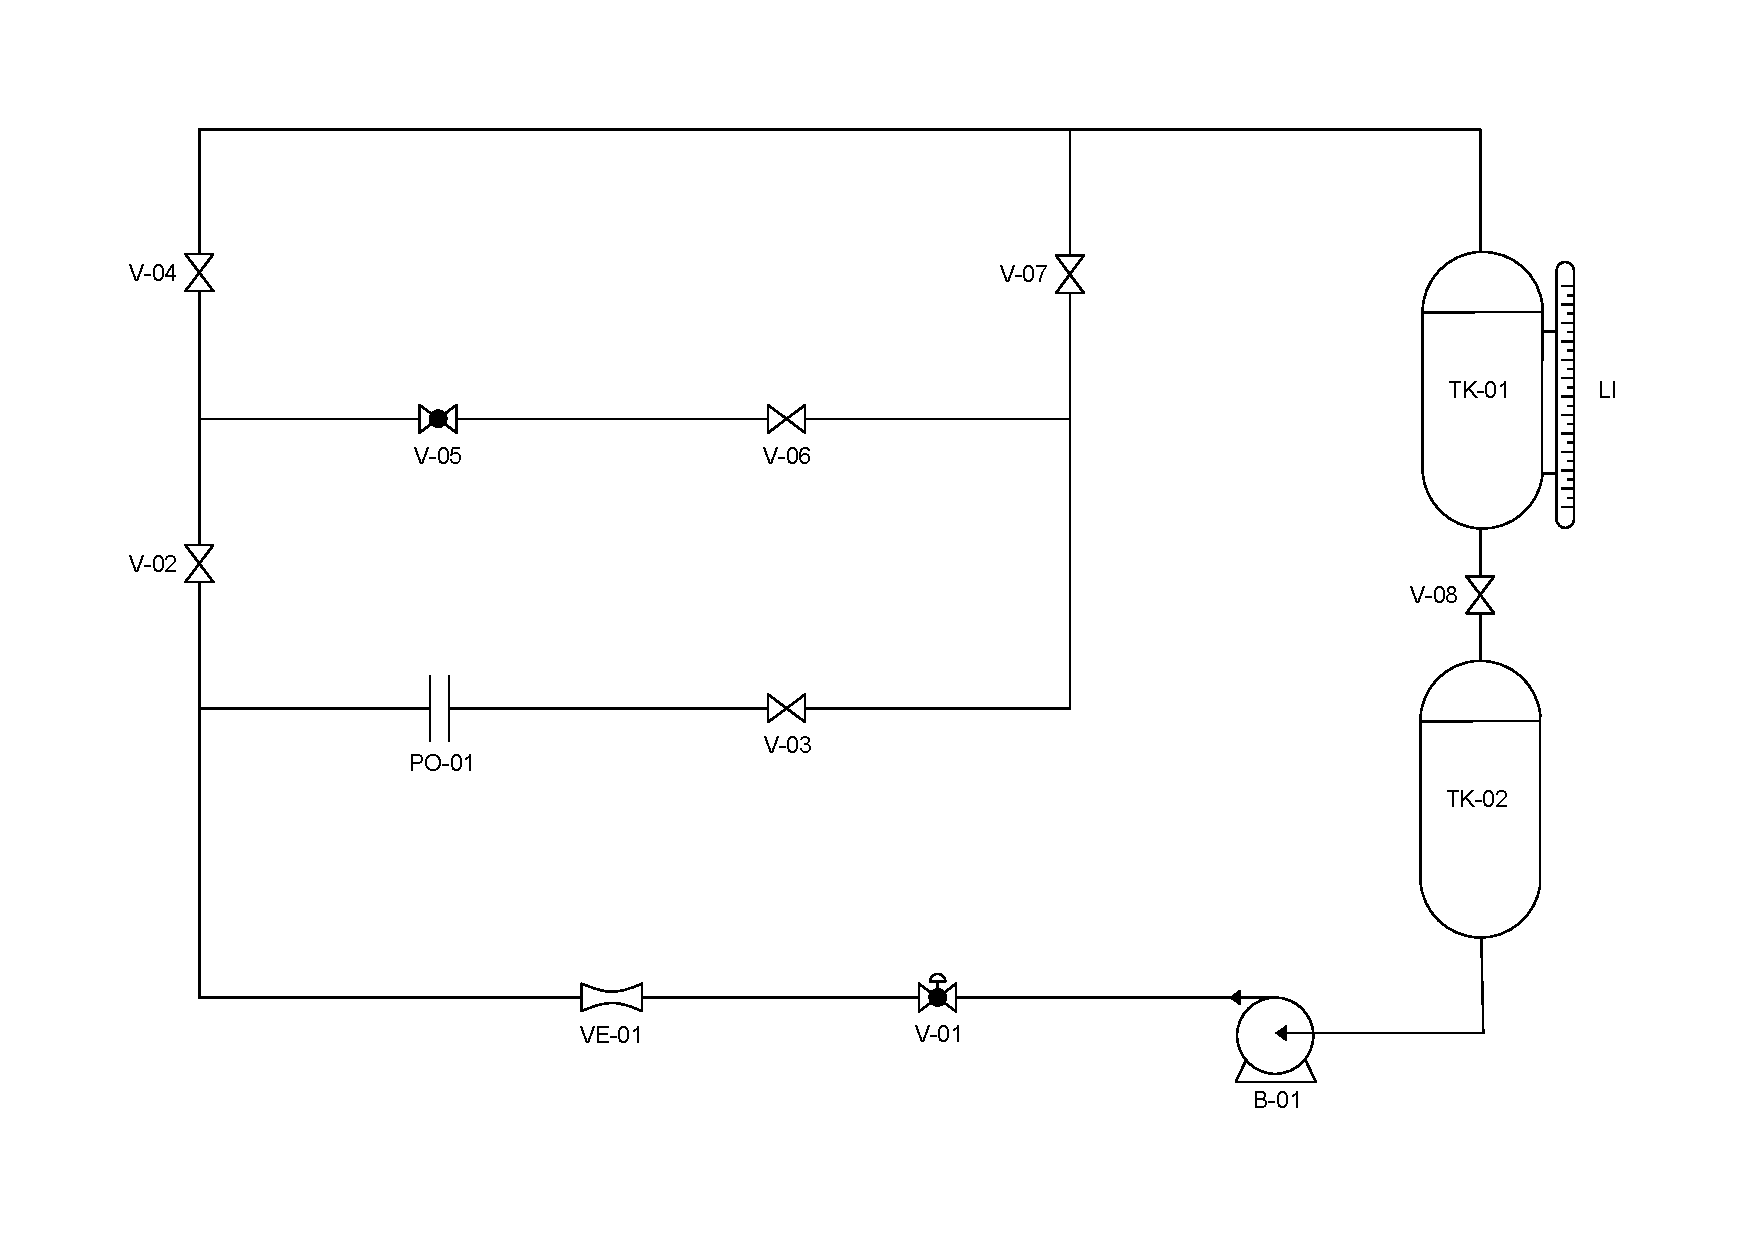
\includegraphics[width=0.8\paperwidth,keepaspectratio]{ensayopc.pdf}}
\end{center}
\caption{Circuito de ensayos de pérdida de carga}
\end{figure}
\subsubsection*{Foto}
\begin{figure}[H]
\begin{center}
\frame{\includegraphics[width=0.8\paperwidth,keepaspectratio]{example-image.jpg}}
\end{center}
\caption{Foto del Circuito de ensayos de pérdida de carga}
\end{figure}
\subsubsection*{Componentes}
\begin{table}[H]
\centering
\begin{tabular}{cp{3.5cm}}
\toprule
Código & Equipo \\
\midrule
B-01 & Bomba \\
\midrule
TK-01 & \multirow{2}{*}{Tanque} \\
TK-02 & \\
\midrule
V-01 & \multirow{2}{*}{Válvula globo} \\
V-05 & \\
\midrule
V-02 & \multirow{5}{*}{Válvula esclusa} \\
V-03 & \\
V-04 & \\
V-06 & \\
V-07 & \\
V-08 & \\
\midrule
PO-01 & Placa orificio \\
\midrule
VE-01 & Tubo Venturi \\
\midrule
LI & Indicador de nivel \\
\bottomrule
\end{tabular}
\end{table}
\subsubsection*{Variables de proceso}
\begin{table}[H]
\centering
\begin{tabular}{cp{3.5cm}}
\toprule
Presión & 0 $barg$ \\
Temperatura & 25\celsius \\
Caudal & $\leqslant 2$ L/s \\
Potencia & No aplica \\
\bottomrule
\end{tabular}
\end{table}
\subsubsection*{Campañas experimentales y resultados}
\begin{itemize}
    \item Pérdida de carga con la placa orificio. Resulta ser mayor que en el Venturi.
    \item Pérdidas de carga con la esclusa parcialmente y completamente cerrada. La válvula abierta tiene menor pérdida de carga.
    \item Pérdida de carga en tramo recto. Se aproxima a los valores teóricos.
\end{itemize}
%\subsubsection*{Experimentos planeados}
%Establecer el desempeño de varios equipos de instrumentación de sodio: transductores nuevos de alta temperatura, transductores ultrasónicos de matriz en fases, transductores electromagnéticos, y también experimentos para demostrar la habilidad de hacer visualización de sodio.

%A largo plazo, DOLMEN será usado para el ensayo de técnicas de reparación de sodio.
\subsubsection*{Actividades de entrenamiento}
No está planificado un programa específico
\newpage
\subsection{CORRONa}
\subsubsection*{Información general}
\textit{Nombre de la instalación: }CORRONa: Corrosion in Sodium (\ce{Na})

\textit{Refrigerante: }Sodio y otros metales líquidos

\textit{Ubicación: }CEA Saclay, Francia

\textit{Inicio de operación: }2010

\subsubsection*{Estado}
En operación

\subsubsection*{Campo de I\&D}
\begin{itemize}
\item[$\square$] Instalación de potencia cero para V \& V y propósitos de licencia
\item[$\square$] Design Basis Accidents (DBA) y Design Extended Conditions (DEC)
\item[$\square$] Termohidráulica
\item[$\square$] Química del refrigerante
\item[$\boxtimes$] Materiales
\item[$\square$] Sistemas y componentes
\item[$\square$] Instrumentación \& ISI\&R
\end{itemize}
\subsubsection*{Descripción técnica}
El sodio líquido (1) está contenido en el crisol de molibdeno (2), que se encuentra en el pozo térmico (3) y es accesible mediante guantes de argón. El pozo es calentado por un horno de alta temperatura desde el exterior (6 $kW$ - 850\celsius) (4). La sección más alta del pozo comprende canales de refrigerante (5) que permiten mantener la temperatura con un valor cercano a la temperatura ambiente mediante la circulación de un refrigerante. El pozo se fija en el piso de la caja de guantes (6) usando una brida de ajuste. Las entradas y salidas de gas (7, 11) se utilizan para el barrido de argón, cuya operación se realiza antes de la prueba, y para el control de la presión cuando el pozo se cierra herméticamente del argón purificado con una tapa (8) durante una prueba de sodio. Esta cubierta se enfría con el mismo refrigerante (10). La temperatura del sodio se mide con termocuplas ubicadas en el pozo térmico (9). Se implementan dos discos de ruptura de 6 barras (14) en la sección superior enfriada del pozo para evitar cualquier posible sobrepresión mientras se mantiene el pozo apretado durante la operación normal. En caso de que esto ocurra, los gases y productos se derivan a una línea de descarga con filtro de aerosoles (13). Los especímenes de corrosión (17) se fijan al condensador con alambre de molibdeno (16).
\subsubsection*{Esquema}
\begin{figure}[H]
\begin{center}
\frame{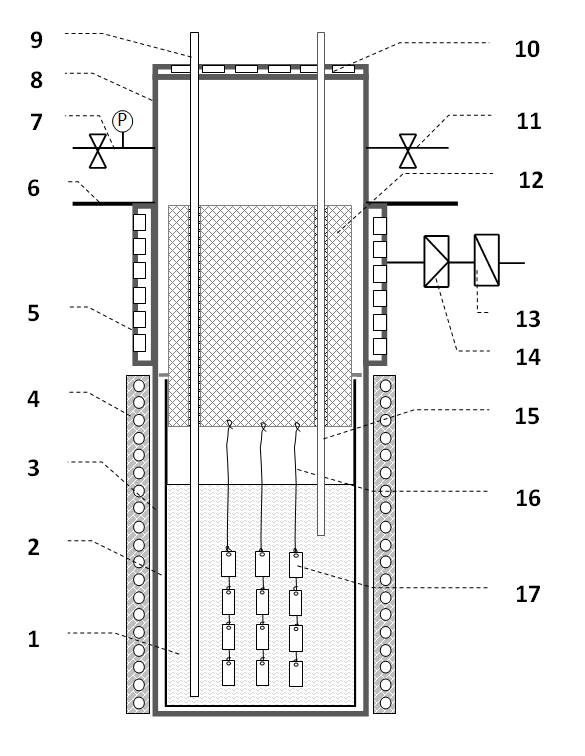
\includegraphics[width=0.45\paperwidth,keepaspectratio]{CORRONa.png}}
\end{center}
\caption{Instalación de corrosión en sodio CORRONa}
\end{figure}
\subsubsection*{Foto}
\begin{figure}[H]
\begin{center}
\frame{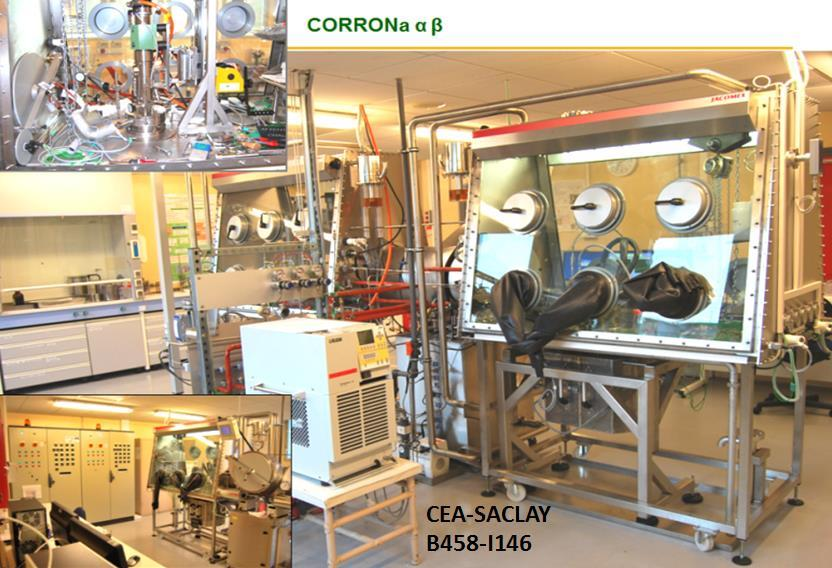
\includegraphics[width=0.8\paperwidth,keepaspectratio]{corrona_photo.jpg}}
\end{center}
\caption{Foto de CORRONa}
\end{figure}
\subsubsection*{Componentes}
\begin{table}[H]
\centering
\begin{tabular}{cp{4cm}}
\toprule
Código & Equipo \\
\midrule
1 & Sodio líquido \\
2 & Crisol de molibdeno \\
3 & Pozo térmico \\
4 & Horno \\
5 & Canales de \newline enfriamiento \\
6 & Piso de caja de guantes \\
7 & Entrada de gas y \newline monitoreo de P \\
8 & Cubierta de pozo \\
9 & Pozo de temperatura \\
10 & Sector de enfriamiento de la cobertura superior \\
11 & Salida de gas \\
12 & Condensador de reflujo de vapor de sodio \\
13 & Filtro de aerosoles \\
14 & Discos de rotura \\
15 & Sensor de oxígeno \\
16 & Cables de molibdeno \\
17 & Espécimen de \newline corrosión \\
\bottomrule
\end{tabular}
\end{table}
\subsubsection*{Variables de proceso}
\begin{table}[H]
\centering
\begin{tabular}{cp{3.5cm}}
\toprule
Presión & 0 $barg$ \\
Temperatura & $\leqslant700\celsius$ \\
Caudal & $\leqslant 1$ m/s \\
Potencia & $2\times6$ $kW$ \\
\bottomrule
\end{tabular}
\end{table}
\subsubsection*{Campañas experimentales y resultados}
\begin{itemize}
    \item Descripción detallada de la oxidación de 316LN y T91.
    \item Cinética a 550\celsius\,en sodio ligeramente oxidante para 316LN y T91
    \item Estudios de los efectos del oxígeno sobre los mecanismos de oxidación a 550\celsius\,en aceros austeníticos
    \item Estudio de la química del sodio y sus comportamientos en sistemas complejos.
    \item Estudios de fragilización de metal líquido
    \item Desarrollo de materiales cerámicos para sensores electroquímicos (oxígeno).
\end{itemize}
%\subsubsection*{Experimentos planeados}
%Establecer el desempeño de varios equipos de instrumentación de sodio: transductores nuevos de alta temperatura, transductores ultrasónicos de matriz en fases, transductores electromagnéticos, y también experimentos para demostrar la habilidad de hacer visualización de sodio.

%A largo plazo, DOLMEN será usado para el ensayo de técnicas de reparación de sodio.
\subsubsection*{Actividades de entrenamiento}
Sólo se planean capacitaciones para estudiantes de MSc y PhD.
\newpage
\subsection{CARNAC}
\subsubsection*{Información general}
\textit{Nombre de la instalación: }CARNAC: Continuous Sodium (\ce{Na}) Carbonation

\textit{Refrigerante: }Sodio

\textit{Ubicación: }CEA Cadarache, Francia

\textit{Inicio de operación: }1998

\subsubsection*{Estado}
En operación

\subsubsection*{Campo de I\&D}
\begin{itemize}
\item[$\square$] Instalación de potencia cero para V \& V y propósitos de licencia
\item[$\square$] Design Basis Accidents (DBA) y Design Extended Conditions (DEC)
\item[$\square$] Termohidráulica
\item[$\boxtimes$] Química del refrigerante
\item[$\square$] Materiales
\item[$\square$] Sistemas y componentes
\item[$\square$] Instrumentación \& ISI\&R
\end{itemize}
\subsubsection*{Descripción técnica}
La instalación de CARNAC fue diseñada para estudiar la transformación química suave del sodio metálico (reacción progresiva) en compuestos químicos más estables en condiciones de temperatura y presión casi normales. Este tipo de proceso es necesario para tratar el sodio metálico residual antes de realizar operaciones de mantenimiento en condiciones de aire, por ejemplo.
\subsubsection*{Esquema}
\begin{figure}[H]
\begin{center}
\frame{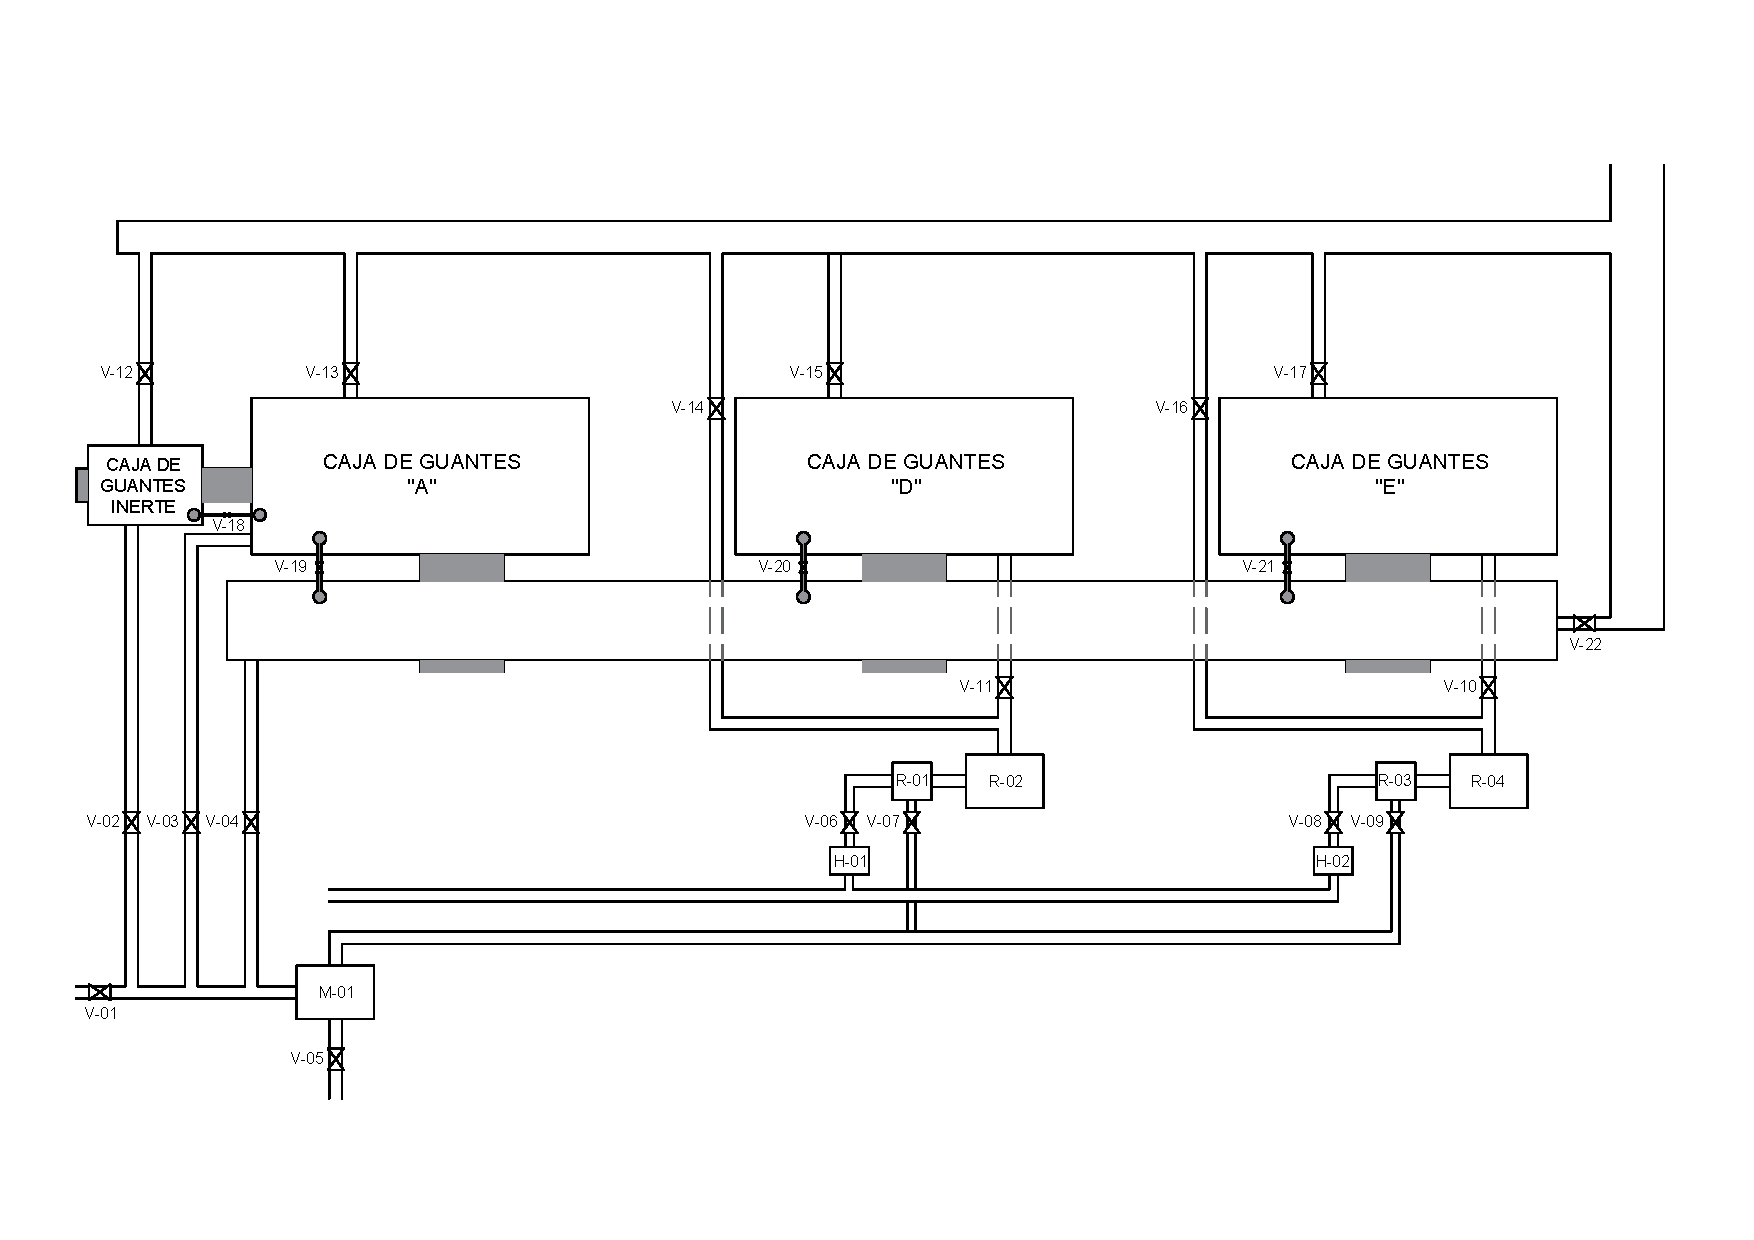
\includegraphics[width=0.8\paperwidth,keepaspectratio]{CARNAC.pdf}}
\end{center}
\caption{Instalación de carbonación de sodio CARNAC}
\end{figure}
\subsubsection*{Foto}
\begin{figure}[H]
\begin{center}
\frame{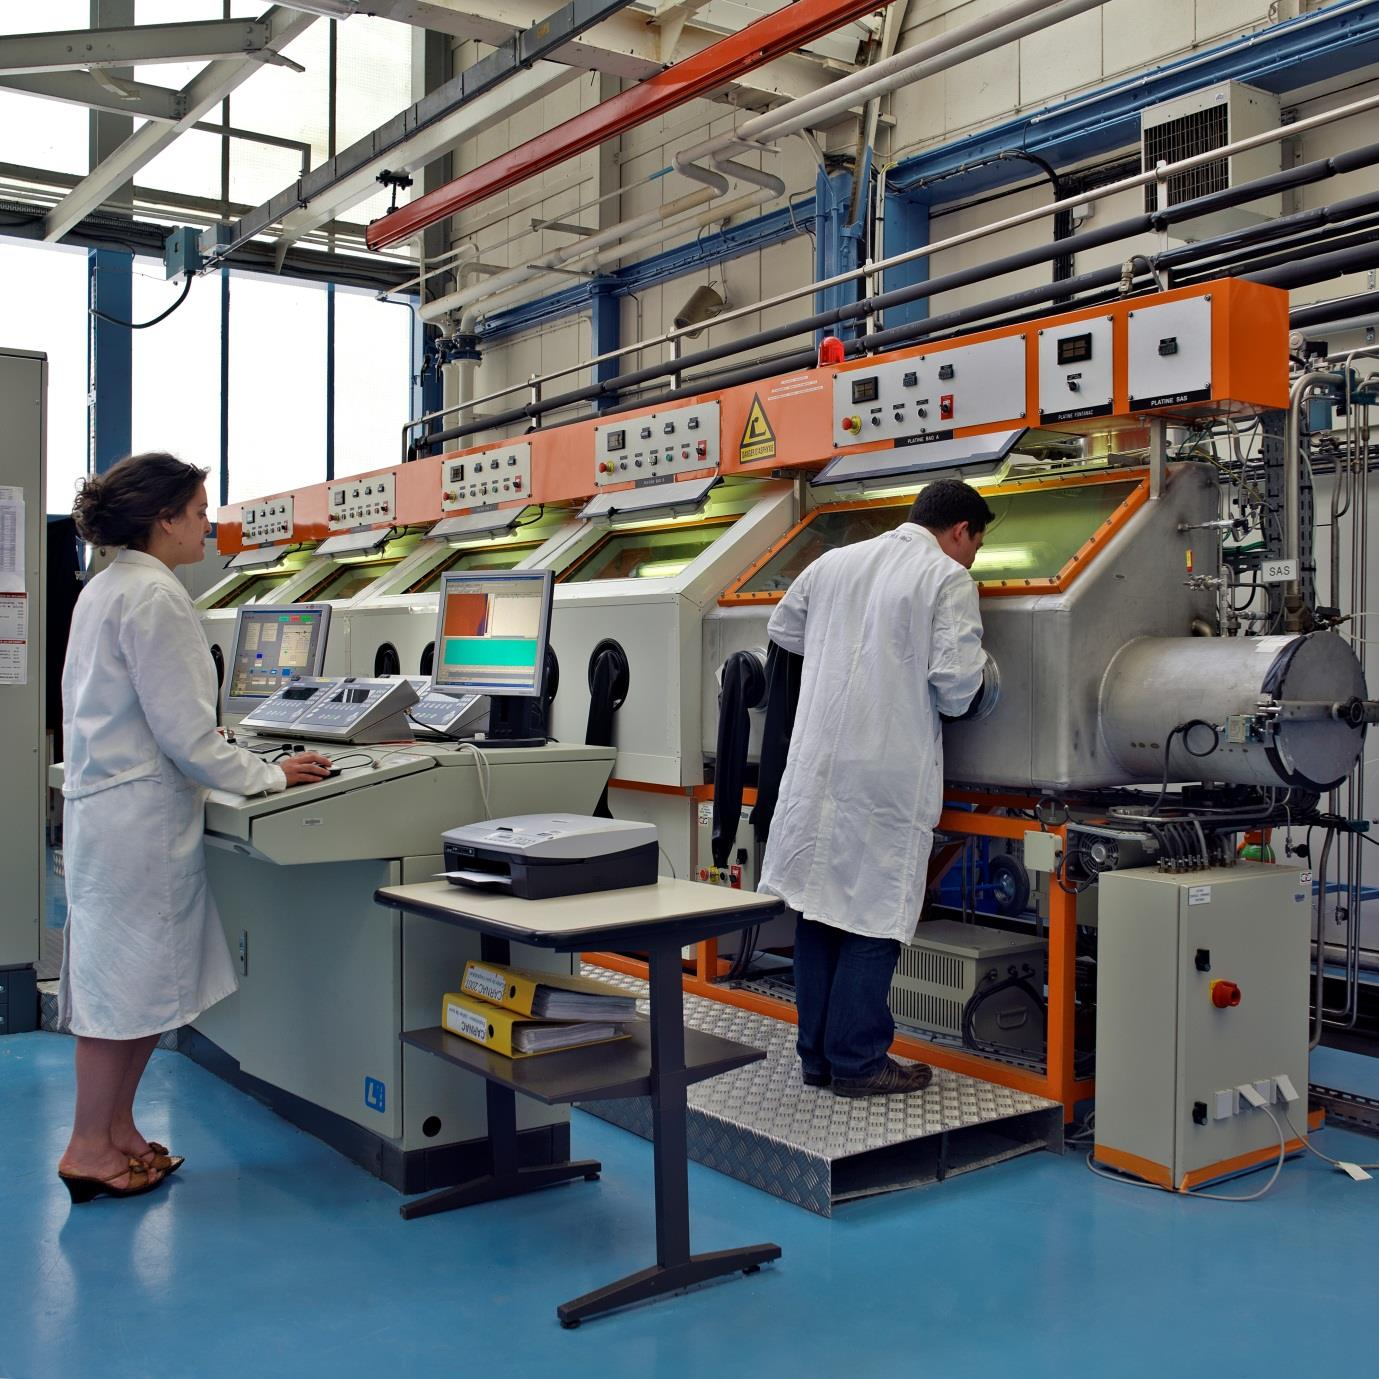
\includegraphics[width=0.8\paperwidth,keepaspectratio]{carnac_photo.jpg}}
\end{center}
\caption{Foto de CARNAC}
\end{figure}
\subsubsection*{Componentes}
\begin{table}[H]
\centering
\begin{tabular}{cp{4cm}}
\toprule
Código & Equipo \\
\midrule
V-01 a V-22 & Válvula esclusa \\
\midrule
R-01 & \multirow{4}{*}{Reservorio} \\
R-02 & \\
R-03 & \\
R-04 & \\
\midrule
H-01 & \multirow{2}{*}{Humidificadores} \\
H-02 & \\
\midrule
M-01 & Mezclador \\
\midrule
& Túnel \\
\midrule
& Caja de guantes A, D y E \\
\midrule
& Caja de guantes inerte \\
\bottomrule
\end{tabular}
\end{table}
\subsubsection*{Variables de proceso}
\begin{table}[H]
\centering
\begin{tabular}{cp{3.5cm}}
\toprule
Presión & 100 $mbarg$ \\
Temperatura & $20\celsius\leqslant T \leqslant60\celsius$ \\
Caudal & $50\frac{L}{h}\leqslant F_v \leqslant10000\frac{L}{h}$ \\
Potencia & No aplica \\
\bottomrule
\end{tabular}
\end{table}
\subsubsection*{Campañas experimentales y resultados}
Originalmente, CARNAC se ha utilizado para el estudio de la carbonatación de sodio (con una mezcla de dióxido de carbono, nitrógeno y vapor de agua). Permite determinar cuál es la mejor mezcla de nitrógeno, dióxido de carbono y vapor de agua para obtener una buena cinética cuando se mantienen los productos de reacción en fase sólida. Estas pruebas han definido:
\begin{itemize}
    \item La influencia de varios parámetros: temperatura, concentraciones de gases de reacción, etc.
    \item Los espesores de sodio carbonatados versus tiempo.
    \item El tipo de carbonatos de sodio que se producen: \ce{NaHCO3} y/o \ce{Na2CO3}
\end{itemize}
Con el conjunto más óptimo de parámetros, el orden de magnitud de la cinética es de aproximadamente 7 mm de sodio metálico tratado en 100 horas. Se realizaron pruebas de carbonatación de larga duración durante más de cuatro meses. Parece que solo hubo una lenta disminución de la cinética, principalmente debido al carbonato de sodio que se expande, se agrieta en todas partes y, por lo tanto, crea nuevas grietas que dan acceso al sodio metálico residual y luego el gas húmedo puede continuar el proceso de carbonatación de sodio.
La optimización de las condiciones de funcionamiento de la carbonatación de sodio en varias configuraciones específicas se ha realizado y aún se está ejecutando. La instalación CARNAC se ha utilizado para estudiar la oxidación del aire natural por el sodio (más o menos húmedo). Se han realizado experimentos como la carbonatación de NaK.
%\subsubsection*{Experimentos planeados}
%Establecer el desempeño de varios equipos de instrumentación de sodio: transductores nuevos de alta temperatura, transductores ultrasónicos de matriz en fases, transductores electromagnéticos, y también experimentos para demostrar la habilidad de hacer visualización de sodio.

%A largo plazo, DOLMEN será usado para el ensayo de técnicas de reparación de sodio.
\subsubsection*{Actividades de entrenamiento}
No se planean capacitaciones
\subsection{Sistema de enfriamiento de Tanque de Blindaje y Blindajes Externos}
\subsubsection*{Información general}
\textit{Nombre de la instalación: }Sistema de enfriamiento de Tanque de Blindaje y Blindajes Externos

\textit{Refrigerante: }Agua liviana

\textit{Ubicación: }Central Nuclear Embalse

\textit{Inicio de operación: }Enero 1984

\subsubsection*{Estado}
En operación

\subsubsection*{Campo de I\&D}

\subsubsection*{Descripción técnica}
A los efectos de disminuir la radiación que se genera en el edificio del Reactor, reducir los daños por radiación de los equipos y cuidar al personal que tiene acceso a dicha parte de la instalación se dispone a la Calandria sumergida en un tanque de hormigón con agua liviana.

El agua del tanque actúa como moderador neutrónico desacelerando los neutrones mediante choques elásticos, lo cual repercute en un descenso en la energía cinética del neutrón pero en una consecuente aumento de la temperatura del medio acuoso.

Por ello, se prevé un sistema de refrigeración del blindaje del reactor a los efectos de remover y disipar la potencia que se genera debido al calentamiento nuclear.
\subsubsection*{Esquema}
\begin{figure}[H]
\begin{center}
\frame{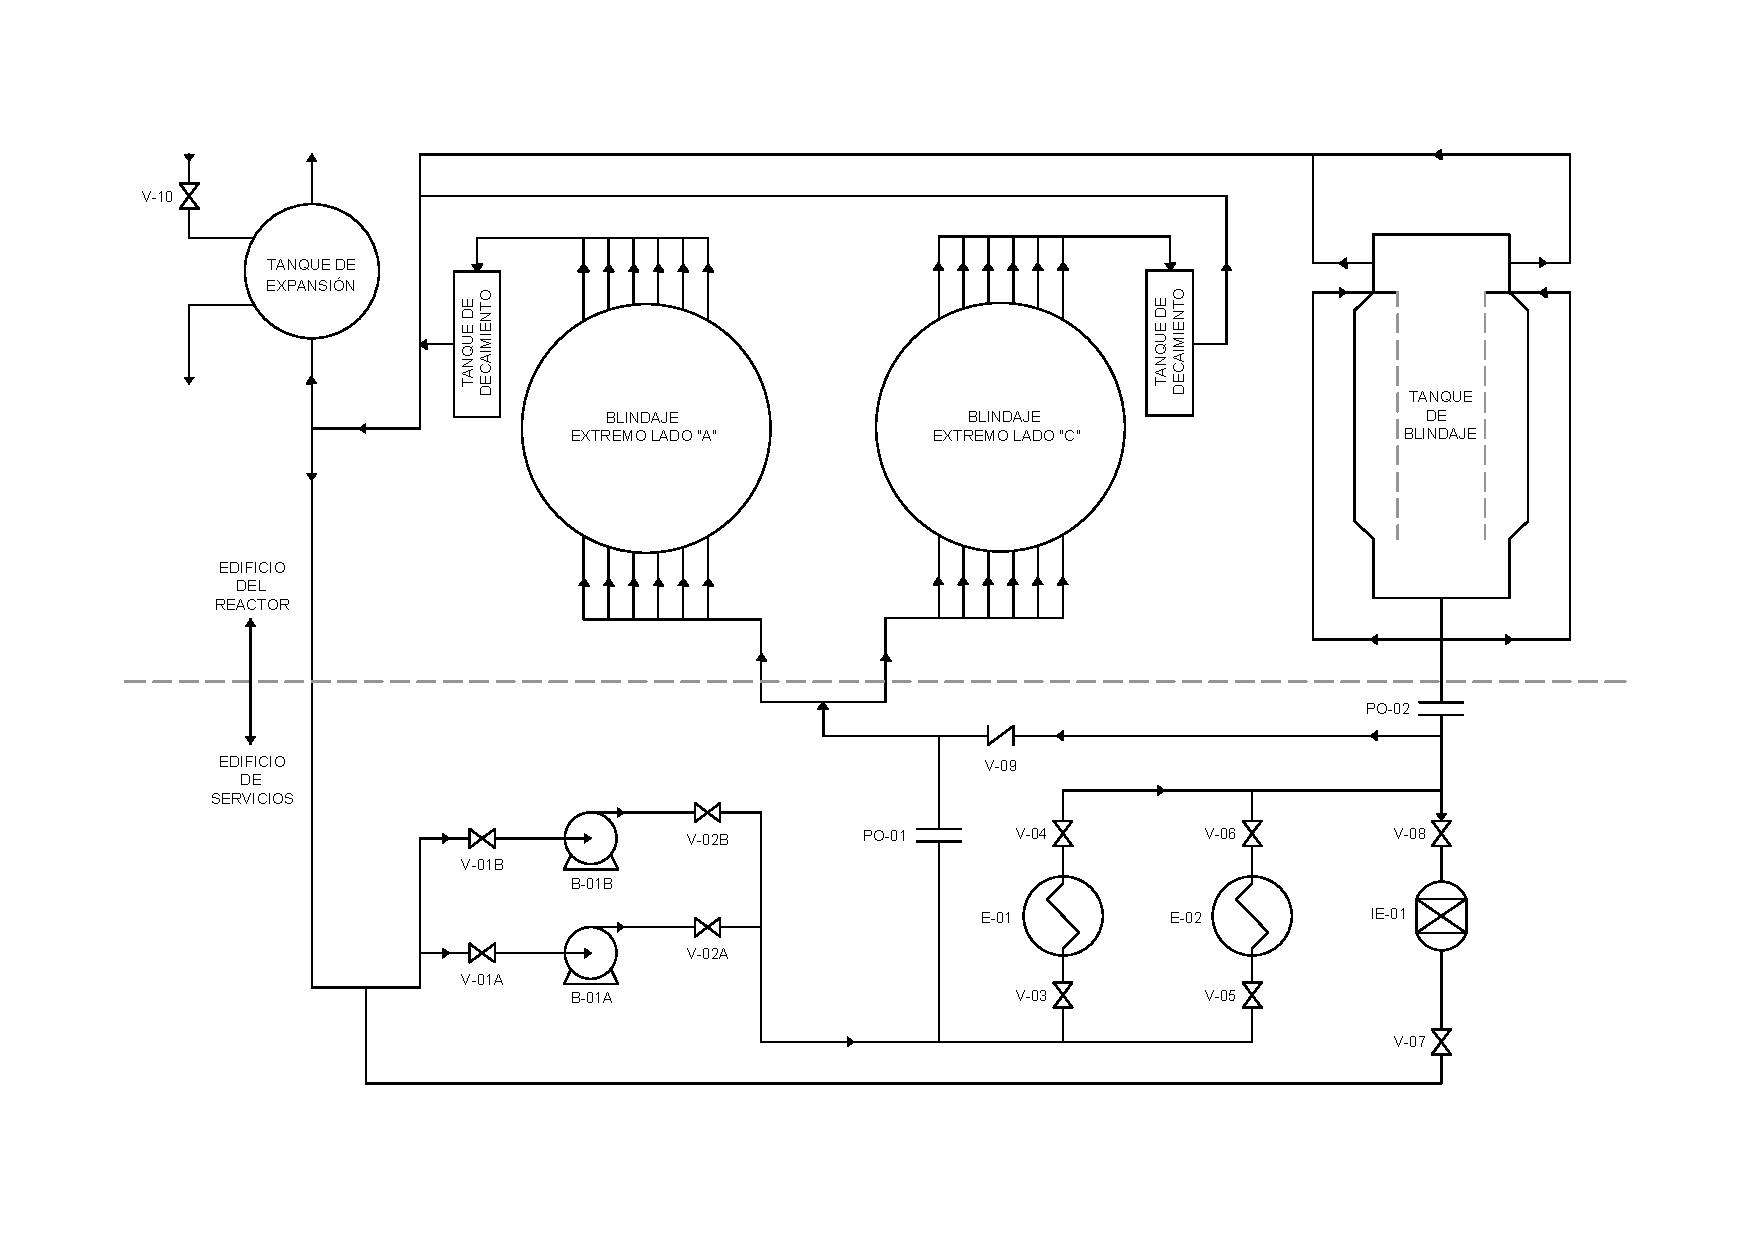
\includegraphics[width=0.8\paperwidth,keepaspectratio]{SIST_ENF.pdf}}
\end{center}
\caption{Sistema de enfriamiento de Tanque de Blindaje y Blindajes Externos}
\end{figure}
\subsubsection*{Foto}
\begin{figure}[H]
\begin{center}
\frame{\includegraphics[width=0.8\paperwidth,keepaspectratio]{example-image.jpg}}
\end{center}
\caption{Foto de la instalación}
\end{figure}
\subsubsection*{Componentes}
\begin{table}[H]
\centering
\begin{tabular}{cp{4cm}}
\toprule
Código & Equipo \\
\midrule
B-01 & \multirow{2}{*}{Bomba de Circulación} \\
B-02 & \\
\midrule
E-01 & \multirow{2}{*}{Intercambiador de calor} \\
E-02 & \\
\midrule
IE-01 & Tanque de Resina de \newline Intercambio Iónico \\
\midrule
& Tanque de Expansión \\
\midrule
& Tanque de decaimiento \\
\bottomrule
\end{tabular}
\end{table}
\subsubsection*{Variables de proceso}
\begin{table}[H]
\centering
\begin{tabular}{cp{3.5cm}}
\toprule
Presión & 0 $barg$ \\
Temperatura & $61\celsius$ (entrada bombas) \\
Caudal & 472 $m^3/h$ \\
Potencia & $6.7$ $MW$ (con reactor funcionando a plena \newline potencia) \\
\bottomrule
\end{tabular}
\end{table}
\subsubsection*{Campañas experimentales y resultados}
No aplica
\subsubsection*{Experimentos planeados}
No aplica
\subsubsection*{Actividades de entrenamiento}
No Aplica
\end{document}
